\documentclass[11pt,a4paper]{article}
\usepackage[margin=2cm]{geometry}
\usepackage[T1]{fontenc}
\usepackage{lmodern}
\usepackage{amsmath,amssymb}
\usepackage{microtype}
\usepackage{tikz}
\usetikzlibrary{arrows.meta,automata,positioning}
\setlength{\parindent}{0pt}
\setlength{\parskip}{4pt}
\setlength{\abovedisplayskip}{5pt}
\setlength{\belowdisplayskip}{5pt}
\pagestyle{empty}
\begin{document}
\begin{center}
{\large\bfseries CSCI 3130 --- HW4: Concise Solutions}
\end{center}

\textbf{Q1.}
$B,C$ are non-generating: every derivation from either retains a $B$ or $C$.
Delete them and $S\to aBB$, leaving
\[
S\to aaA,\qquad A\to aA\mid\lambda.
\]
Eliminating $A\to\lambda$ gives
\[
\boxed{S\to aaA\mid aa,\qquad A\to aA\mid a.}
\]
There are no unit-, useless-, or $\lambda$-productions.
Since originally $A$ generates $a^*$, $\boxed{L=\{a^n:n\ge2\}}$.

\medskip
\textbf{Q2.}
No $\lambda$- or unit-productions occur; all variables are generating and reachable.

Introduce $X\to a$ and $Y\to b$. Replacing terminals in longer rules gives
\[
A\to XAB\mid b,\qquad B\to YB\mid YAC
\quad(S,C\text{ unchanged}).
\]
Introduce $D\to AB$ and $E\to AC$ to split the length-three rules.
The final CNF grammar is
\[
\boxed{\begin{aligned}
S&\to AB\mid a, & C&\to c,\\
A&\to XD\mid b, & D&\to AB,\\
B&\to YB\mid YE, & E&\to AC,\\
X&\to a, & Y&\to b.
\end{aligned}}
\]
Every rule has the form $U\to VW$ or $U\to t$.

\medskip
\textbf{Q3.}
\textbf{(1) Deterministic.} Each transition set is a singleton.
The $a$-move requires stack top $z$, whereas the $\lambda$-move requires $A$;
they cannot be enabled together.

\textbf{(2) Nondeterministic.}
At $(q_0,z)$ with next input $a$, both $\delta(q_0,a,z)$ and
$\delta(q_0,\lambda,z)$ are enabled, violating DPDA determinism.

\medskip
\textbf{Q4.}
Use $Q=\{q_0,q_1,q_f\}$, $\Sigma=\{a,b,c\}$, $\Gamma=\{A,Z_0\}$.
Start in $q_0$ with stack $Z_0$; $F=\{q_f\}$.
Labels $x,X\to\gamma$ mean read $x$ and replace top $X$ by $\gamma$
(leftmost symbol on top). All unshown transitions are empty.

\begin{center}
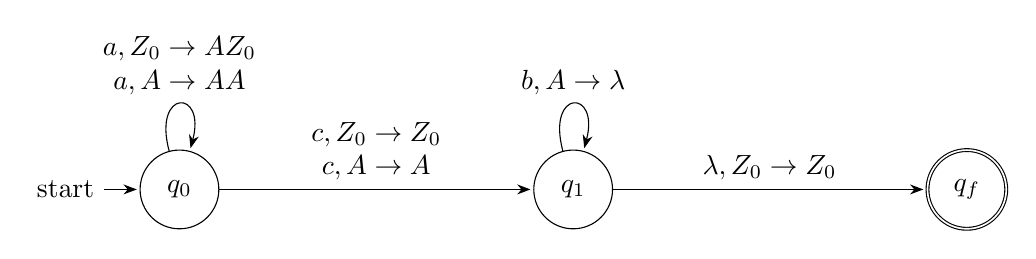
\begin{tikzpicture}[
  >=Stealth,shorten >=1pt,node distance=5cm,on grid,auto,
  every state/.style={minimum size=10mm},
  every edge/.style={draw,->},initial text={start}
]
\node[state,initial] (q0) {$q_0$};
\node[state,right=of q0] (q1) {$q_1$};
\node[state,accepting,right=of q1] (qf) {$q_f$};
\path
  (q0) edge[loop above] node[align=center]
    {$a,Z_0\to AZ_0$\\$a,A\to AA$} (q0)
  (q0) edge node[align=center]
    {$c,Z_0\to Z_0$\\$c,A\to A$} (q1)
  (q1) edge[loop above] node {$b,A\to\lambda$} (q1)
  (q1) edge node {$\lambda,Z_0\to Z_0$} (qf);
\end{tikzpicture}
\end{center}

Each $a$ pushes one $A$; after the unique $c$, each $b$ pops one $A$.
Acceptance requires reaching $q_f$ with all input consumed, hence equal numbers
of $a$'s and $b$'s. For $n=0$, $c$ is also accepted. Thus $L(M)=\{a^ncb^n:n\ge0\}$.
\end{document}
